
\subsection{Long short-term memory} 

\textit{Long short-term memory} (LSTM) were proposed (1997) by Hochreiter and Schmidhuber\cite{lstm} as a novel network 
structure to address the vanishing gradient problem, which was first studied by Hochreiter (1991) in his diploma 
thesis, a milestone of deep learning.

The idea behind this structure is to enforce a constant error flow, that is to say, to have constant gradient norm, 
thus preventing the gradient to vanish. This is done by introducing special types of neurons called \textit{memory 
cells} and \textit{gate units}. As we can see by looking at figure \ref{lstm_neuron}, a memory cell is essentially a 
neuron with a self connection with unitary weight, whose input and output are managed by two multiplicative neurons: 
the gate units.


\tikzstyle{nn_style}=[->,shorten >=1pt,auto,node distance=1.5cm,
  thick,
  neuron/.style={circle,fill=white!50,node distance=1cm,draw,minimum size=0.7cm,font=\sffamily\normalsize},
  missing/.style={circle,font=\sffamily\Large,node distance=0.95cm},
  label/.style={node distance=1.2cm,rectangle,fill=white!50,draw=none,minimum size=0.7cm,font=\sffamily\normalsize},
  layer/.style={rectangle,fill=white!50,draw,minimum width=0.8cm,font=\sffamily\Large},
  loopStyle/.style={in=120,out=60, distance=2.5cm},
  weight/.style = {above,sloped,pos=0.3},]
\begin{figure}[h]
  \centering
  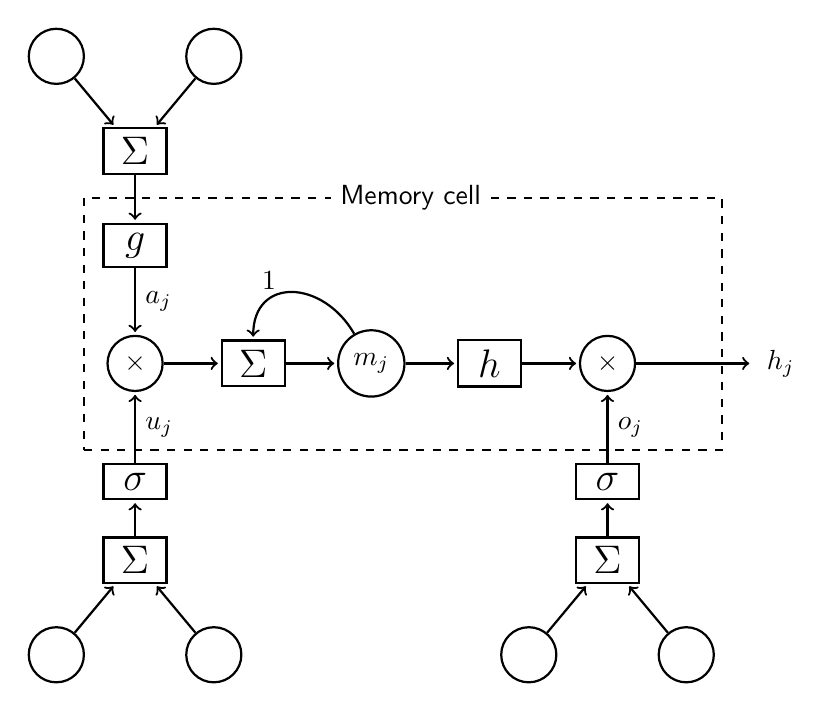
\begin{tikzpicture}[nn_style]

    %horizontal line
    \node[neuron]	(c1)       					{$\times$};
    \node[layer] 	(s_mem)	[right of=c1,	node distance=1.5cm] 	{$\Sigma$};
    \node[neuron]	(mem)	[right of=s_mem,node distance=1.5cm]	{$m_j$};
    \node[layer] 	(h)	[right of=mem,	node distance=1.5cm] 	{$h$};
    \node[neuron]	(c2)	[right of =h,	node distance=1.5cm]	{$\times$};
    \node[label]  	(out)	[right of=c2,	node distance=2.2cm]	{$h_j$};
    
    \path[->] (c1) 	edge []   (s_mem)
	      (s_mem) 	edge []   (mem)
	      (mem) 	edge []   (h)
	      (h) 	edge []   (c2)
	      (c2) 	edge []   (out);
	     
    
    %loop	     
    \path[->] (mem) edge [loop, in=90,out=120, distance=0.8cm, anchor=south ] node [align=center, pos=0.7] 
 {$1$} (s_mem);

    
    %above inputs
    \node[layer] 	(g)	[above of=c1,	node distance=1.5cm] 	{$g$};
    \node[layer] 	(s_in)	[above of=g,	node distance=1.2cm] 	{$\Sigma$};
    \node[missing]	(i2)	[above of=s_in, node distance=1.2cm]	{$\hdots$};
    \node[neuron]	(i3)	[right of=i2, 	node distance=1cm]	{};
    \node[neuron]	(i1)	[left of=i2, 	node distance=1cm]	{};

    
    \path[->] (s_in) 	edge [anchor=west]	node[]{}	(g)
	      (g) 	edge [anchor=west]   	node[]{$a_j$}	(c1)
	      (i1)	edge []   					(s_in) 
      	      (i3)	edge []   					(s_in);
      	      
      	      
    %below gate input unit
    \node[layer] 	(sig_in)	[below of=c1,		node distance=1.5cm] 	{$\sigma$};
    \node[layer] 	(s_gate_in)	[below of=sig_in,	node distance=1cm] 	{$\Sigma$};
    \node[missing]	(gi2)		[below of=s_gate_in, 	node distance=1.2cm]	{$\hdots$};
    \node[neuron]	(gi3)		[right of=gi2, 		node distance=1cm]	{};
    \node[neuron]	(gi1)		[left of=gi2, 		node distance=1cm]	{};

    
    \path[->] (s_gate_in) 	edge [anchor=west]	node[]{}	(sig_in)
	      (sig_in) 		edge [anchor=west]	node[]{$u_j$} 	(c1)
	      (gi1)		edge []   (s_gate_in) 
      	      (gi3)		edge []   (s_gate_in);
      	      
      	      
    %below gate output unit
    \node[layer] 	(sig_out)	[below of=c2,		node distance=1.5cm] 	{$\sigma$};
    \node[layer] 	(s_gate_out)	[below of=sig_out,	node distance=1cm] 	{$\Sigma$};
    \node[missing]	(go2)		[below of=s_gate_out, 	node distance=1.2cm]	{$\hdots$};
    \node[neuron]	(go3)		[right of=go2, 		node distance=1cm]	{};
    \node[neuron]	(go1)		[left of=go2, 		node distance=1cm]	{};

    
    \path[->] (s_gate_out) 	edge [anchor=west]	node[]{}	   (sig_out)
	      (sig_out) 	edge [anchor=west]	node[]{$o_j$}   (c2)
	      (go1)		edge []						   (s_gate_out) 
      	      (go3)		edge []						   (s_gate_out);

    %enclosing rectangle
    \node[rectangle,dashed,fill=none,draw,minimum height=3.2cm,minimum width=8.1cm] at (3.4, 0.5) (memoryCell)	{};
    \node[label]  (memoryLabel)	at(3.5,2.1)	{Memory cell};


      	      
\end{tikzpicture}
\caption{Memory cell and gate units of LSTM network}
\label{lstm_neuron}
\end{figure}

The memory cell and the gate units behave accordingly to the following:

\begin{align}
&u_j^t = \sigma[\mat{W_u}\cdot\vec{x_t} + \mat{U}_u\cdot\vec{h}_{t-1}]_j \\
&o_j^t = \sigma[\mat{W_o}\cdot\vec{x_t} + \mat{U}_o\cdot\vec{h}_{t-1}]_j \\
&a^t_j\defeq g[\mat{W}\cdot\vec{x_t} + \mat{U}\cdot h_i^t]_j\\
\label{mem_update}
&m_j^t\defeq a_j\cdot u_j^t + (1 \cdot m_j^{t-1})\\
&h_j\defeq h(m_j^t)\cdot o^t_j
\end{align}


% \begin{equation}
% u^t_j\defeq \sigma(\sum_i w_{ui}\cdot u^{t-1}_j)
% \end{equation}
% \begin{equation}
% o^t_j\defeq \sigma(\sum_i w_{oi}\cdot o^{t-1}_j)
% \end{equation}
% 
% 
% \begin{equation}
% a^t_j\defeq g(\sum_i w_{ij}\cdot \phi_i^t)
% \end{equation}
% \begin{equation}
%  m_j^t\defeq a_j\cdot u_j^t + (1 \cdot m_j^{t-1})
% \label{mem_update}
% \end{equation}
% \begin{equation}
%  \phi_j\defeq h(m_j^t)\cdot o^t_j
% \end{equation}

As we can see from equation \ref{mem_update}, the value of the memory cell $m(t)$ remains constant as long as the input 
gate $u$ doesn't ``open'' causing a ``write'' operation. Similarly the output $o$ of the memory cell, which is 
connected with 
the other neurons of the network, is controlled by an output gate: the memory will have a non zero output only if the 
output gate opens, which we could call a  a ``read'' operation. As for constant error flow it is ensured because the 
memory cell has only a self-loop with unitary weight.

Memory cells, guarded by gate units can be employed in networks with various topology alongside traditionally 
input, output and hidden units. Another way to look at this kind of architecture is to think of memory cells as units 
able to store one bit of information, even for long periods of time, hence able to learn distant time correlations 
between inputs.

As we have seen these network units are specifically designed to store information, through the use of gates; these 
gates however are no different from other units, apart from the fact they are multiplicative units, hence without 
further precautions, the networks would incur in the same vanishing problem it aimed to resolve. In fact LSTM comes with 
a proper learning algorithm: essentially errors arriving at memory cells inputs are not propagated back in time, only 
the error within the memory cell gets propagated; in other words gradients are truncated taking into account only the 
self-connection of the memory cells and not it's other input connections, hence providing constant error flow.
\\\\
LSTM units have proven to be very successful reaching state-of-art results in various tasks and even at present times 
(2015), they continue to be largely
employed. In recent implementations however, alongside small modifications, as the introduction of other gates, LSTM 
architecture is often used without the original learning algorithm which is often replaced by a standard stochastic 
gradient descend as done in \cite{lstmGraves}.







